% EM-Bayesian G-BVAR — how it differs. Standalone TikZ -> PDF -> PNG.
\documentclass[border=10pt]{standalone}
\usepackage[T1]{fontenc}
\usepackage{helvet}
\renewcommand{\familydefault}{\sfdefault}
\usepackage{amsmath,amssymb,bm}
\usepackage{tikz}
\usetikzlibrary{arrows.meta,positioning,calc,shapes.geometric,fit,backgrounds}

\definecolor{MadridBlue}{RGB}{28,54,99}
\definecolor{MadridBlue2}{RGB}{48,91,150}
\definecolor{Ink}{RGB}{35,35,35}
\definecolor{Muted}{RGB}{105,105,105}
\definecolor{LightGrey}{RGB}{244,245,247}
\definecolor{MidGrey}{RGB}{210,214,221}
\definecolor{SoftBlue}{RGB}{235,241,249}
\definecolor{SoftBlue2}{RGB}{224,233,246}
\definecolor{AccentRed}{RGB}{150,45,45}
\definecolor{CheckGreen}{RGB}{39,116,75}

\tikzset{
  emstep/.style={rounded corners=3pt, draw=MadridBlue, line width=0.9pt, fill=SoftBlue,
    text=Ink, align=center, inner sep=6pt, font=\footnotesize, text width=3.5cm, minimum height=1.35cm},
  emE/.style={emstep, fill=SoftBlue2},
  proc/.style={rounded corners=3pt, draw=MadridBlue, line width=0.9pt, fill=LightGrey,
    text=Ink, align=center, inner sep=7pt, font=\small},
  solve/.style={proc, fill=SoftBlue, draw=MadridBlue, line width=1.4pt},
  usbox/.style={rounded corners=3pt, draw=MadridBlue, line width=1.2pt, fill=MadridBlue,
    text=white, align=center, inner sep=6pt, font=\footnotesize, text width=3.6cm, minimum height=1.3cm},
  greentag/.style={rounded corners=2pt, draw=CheckGreen, line width=0.8pt, fill=white,
    text=CheckGreen, align=left, font=\scriptsize, inner sep=4pt},
  note/.style={align=center, font=\scriptsize, text=Muted, inner sep=2pt},
  flowarr/.style={-{Stealth[length=2.6mm]}, draw=MadridBlue2, line width=1.0pt},
  looparr/.style={-{Stealth[length=3mm]}, draw=AccentRed, line width=1.2pt},
  fb/.style={-{Stealth[length=2.6mm]}, draw=MadridBlue2, line width=1.1pt},
}

\begin{document}
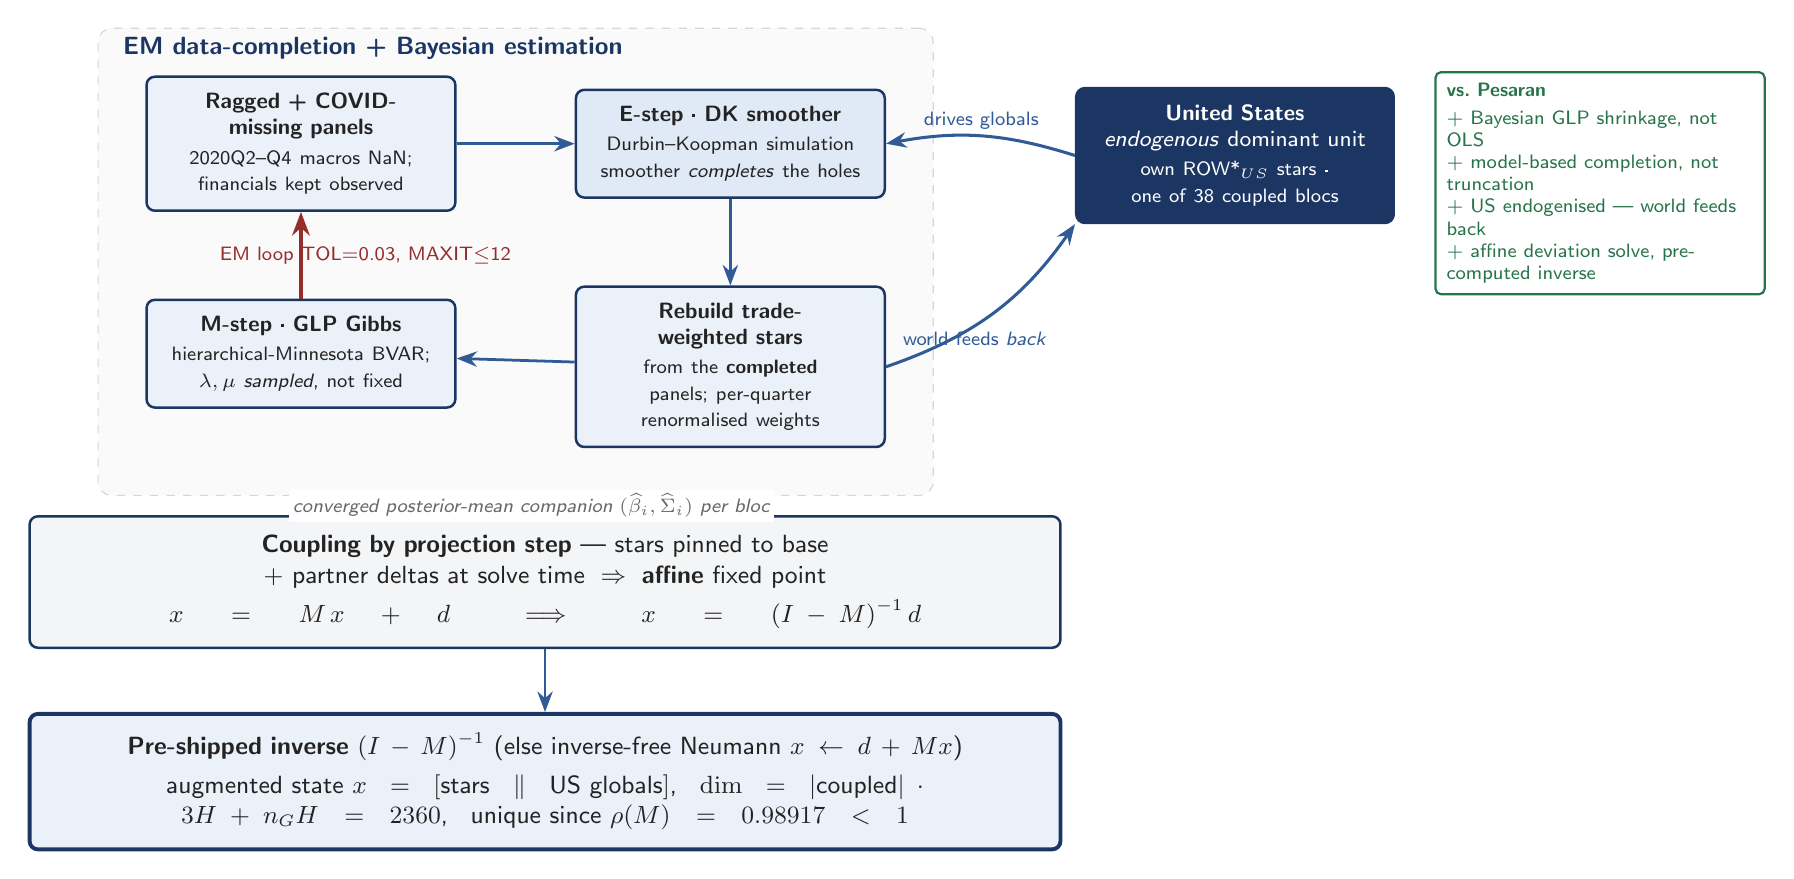
\begin{tikzpicture}

% ================= EM completion loop (left cluster) =================
\node[emstep] (panel) {\textbf{Ragged + COVID-missing panels}\\[1pt]
   {\scriptsize 2020Q2--Q4 macros NaN; financials kept observed}};
\node[emE, right=1.5cm of panel] (dk) {\textbf{E-step · DK smoother}\\[1pt]
   {\scriptsize Durbin--Koopman simulation smoother \emph{completes} the holes}};
\node[emstep, below=1.1cm of dk] (rebuild) {\textbf{Rebuild trade-weighted stars}\\[1pt]
   {\scriptsize from the \textbf{completed} panels; per-quarter renormalised weights}};
\node[emstep, below=1.1cm of panel] (glp) {\textbf{M-step · GLP Gibbs}\\[1pt]
   {\scriptsize hierarchical-Minnesota BVAR; $\lambda,\mu$ \emph{sampled}, not fixed}};

% cycle arrows
\draw[flowarr] (panel) -- (dk);
\draw[flowarr] (dk) -- (rebuild);
\draw[flowarr] (rebuild) -- (glp);
\draw[looparr] (glp) -- node[left,note,text=AccentRed]{EM loop}
                          node[right,note,text=AccentRed]{\!\!TOL$=$0.03, MAXIT$\le$12} (panel);

% group box behind the loop
\begin{scope}[on background layer]
\node[draw=MidGrey, dashed, rounded corners=5pt, fit=(panel)(dk)(rebuild)(glp),
      inner sep=6mm, fill=LightGrey!45] (loopbox) {};
\end{scope}
\node[anchor=north west, font=\small\bfseries, text=MadridBlue] at (loopbox.north west)
  {\hspace{2mm}EM data-completion + Bayesian estimation};

% ================= endogenous US =================
\node[usbox, right=2.4cm of dk, yshift=-0.15cm] (us)
  {\textbf{United States}\\ \emph{endogenous} dominant unit\\[1pt]
   {\scriptsize own ROW*$_{US}$ stars · one of 38 coupled blocs}};
\draw[fb] (us.west) to[bend right=14] node[above,note,text=MadridBlue2]{drives globals} (dk.east);
\draw[fb] (rebuild.east) to[bend right=18] node[below,note,text=MadridBlue2,pos=0.4]{world feeds \emph{back}} (us.south west);

% ================= the affine coupled solve =================
\node[proc, below=1.35cm of glp, text width=12.6cm, xshift=3.1cm] (fixed)
  {\textbf{Coupling by projection step} — stars pinned to base $+$ partner deltas at solve time \;$\Rightarrow$\; \textbf{affine} fixed point\\[3pt]
   $\displaystyle x \;=\; M\,x \;+\; d
      \qquad\Longrightarrow\qquad x \;=\; (I-M)^{-1}\,d$};

\node[solve, below=8mm of fixed, text width=12.6cm] (solve)
  {\textbf{Pre-shipped inverse} $(I-M)^{-1}$ (else inverse-free Neumann $x\!\leftarrow\! d+Mx$)\\[3pt]
   {\small augmented state $x=[\text{stars}\;\|\;\text{US globals}]$,\;\; $\dim=|\text{coupled}|\cdot 3H+n_G H = 2360$,\;\; unique since $\rho(M)=0.98917<1$}};

\draw[flowarr] (loopbox.south) to[out=-90,in=90]
  node[pos=0.52, fill=white, inner sep=1.5pt, font=\scriptsize\itshape, text=Muted]
  {converged posterior-mean companion $(\widehat{\beta}_i,\widehat{\Sigma}_i)$ per bloc} (fixed.north);
\draw[flowarr] (fixed.south) -- (solve.north);

% ================= green contrast tags =================
\node[greentag, right=5mm of us.north east, anchor=north west, text width=3.9cm, yshift=0.2cm] (t1)
  {\textbf{vs.\ Pesaran}\\[2pt]
   \textcolor{CheckGreen}{$+$} Bayesian GLP shrinkage, not OLS\\
   \textcolor{CheckGreen}{$+$} model-based completion, not truncation\\
   \textcolor{CheckGreen}{$+$} US endogenised — world feeds back\\
   \textcolor{CheckGreen}{$+$} affine deviation solve, pre-computed inverse};

\end{tikzpicture}
\end{document}
